\documentclass[aspectratio=169]{beamer}
\usepackage{graphicx} % Required for inserting images
\usepackage{colortbl}
\usepackage{adjustbox}
\usepackage{mathtools}
\usepackage{hhline}

\usepackage{listings}
\usepackage{color}
\usepackage{natbib}
\usepackage{xcolor}

\graphicspath{ {./images/} }

\title{
	Bualoi Production Milestone 2
}
\subtitle{
    Project Proposal Group 11
}

\author{
   BualoiDev 
}
\date{
%2024
}
\beamertemplatenavigationsymbolsempty

\usetheme{Antibes}


\AtBeginSection[]{
\begin{frame}
  \vfill
  \centering
  \begin{beamercolorbox}[sep=8pt,center,shadow=true,rounded=true]{title}
    \usebeamerfont{title}\insertsectionhead\par%
  \end{beamercolorbox}
  \vfill
  \end{frame}
}

\addtobeamertemplate{navigation symbols}{}{%
    \usebeamerfont{footline}%
    \usebeamercolor[fg]{footline}%
    \hspace{1em}%
    \insertframenumber/\inserttotalframenumber
}

\begin{document}

\frame{\titlepage}

\section{Member}
\begin{frame}{Member}
    \begin{enumerate}
        \item Nasmeen Islam
        \item Tanadol Jaichuen
        \item Wiroonpuri Silasap
        \item Kawin Rattanapun
        \item Tanaphom Hirunyathorn
        \item Chawanakorn Auckayachinda
        \item Paponthanai Ounsopa
        \item Nontanun Ausungnoen
        \item Pana Wanitchollakit
    \end{enumerate}
\end{frame}

\begin{frame}{Table of contents}
    \only<1>{\tableofcontents[sections={1-3}]}
    \only<2>{\tableofcontents[sections={4-}]}
\end{frame}

\section{Introduction}

\begin{frame}
    \centering
    
\includegraphics[width=0.75\textwidth]{intro.png} \\
    37,810M Baht, 1.159T Baht

\end{frame}

\begin{frame}
    \centering
    
\includegraphics[width=0.8\textwidth]{example0.png}
\end{frame}

\begin{frame}
    \centering
    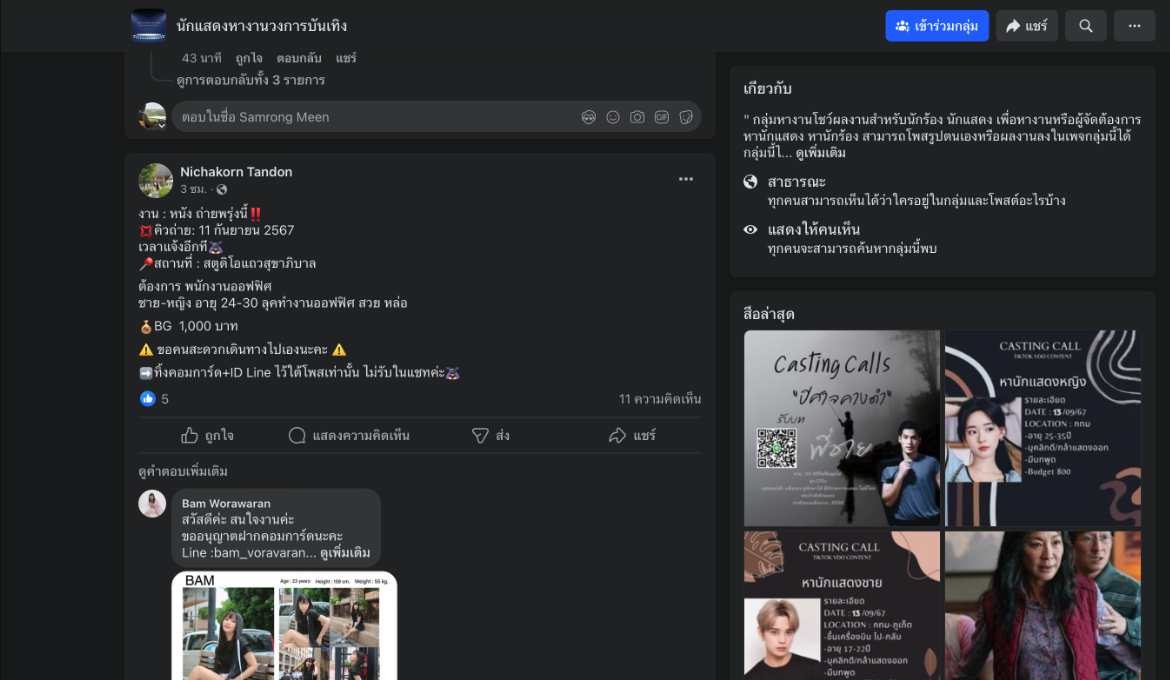
\includegraphics[width=0.8\textwidth]{example1.png}
\end{frame}

\subsection{Organization background}

\begin{frame}{Organization background}
    Bualoi Production
    \begin{enumerate}
        \item Support the creation of new networks and collaborations within the industry
        \item Address inefficiencies in the media and film production industry by improving the connection between media producers and directors.
        \item Enable professionals in the industry to showcase their work and skills, expanding access to diverse job opportunities.
    \end{enumerate}
\end{frame}

\subsection{Problem Statement}

\begin{frame}{Problem Statement}
    1. Interest in Media Production
    \begin{alertblock}{Problem}
        There are significant challenges in finding or accessing sources for media production.
    \end{alertblock}

    \begin{block}{Cause \& Effect}
        Limited access to databases or networks leads to wasted time and risks finding suitable teams.
    \end{block}

    \begin{exampleblock}{Solution}
        Develop a platform for connecting with media producers.
    \end{exampleblock}
\end{frame}

\begin{frame}{Problem Statement}
    2. Contracts or Agreements Lack Clarity
    \begin{alertblock}{Problem}
        Contracts or agreements often have misunderstandings.
    \end{alertblock}

    \begin{block}{Cause \& Effect}
        A lack of standards and communication leads to strained relationships and legal complications.
    \end{block}

    \begin{exampleblock}{Solution}
        Create standardized contract templates and prepare tools to facilitate clear agreements.
    \end{exampleblock}

\end{frame}

\begin{frame}{Problem Statement}
    3. Finding Team Members or Showcasing Skills
    \begin{alertblock}{Problem}
        It is challenging to present skills and reliability to employers.
    \end{alertblock}

    \begin{block}{Cause \& Effect}
        The difficulty in showcasing skills leads to fewer opportunities in the media production industry.
    \end{block}

    \begin{exampleblock}{Solution}
        Create a searchable database that allows sorting based on the specific skills and attributes required.
    \end{exampleblock}

\end{frame}

\begin{frame}{Problem Statement}
    4. Concerns Over the Quality of Production
    \begin{alertblock}{Problem}
        There are concerns regarding transparency, competency, and reliability in production quality.
    \end{alertblock}

    \begin{block}{Cause \& Effect}
        A lack of trustworthy sources leads to doubts or risks in production quality.
    \end{block}

    \begin{exampleblock}{Solution}
        Enable third-party certification uploads, verification, and customer reviews to track performance.
    \end{exampleblock}

\end{frame}

\subsection{Definition}
\begin{frame}{Definition}

    \begin{table}[ht]
        \centering
        \begin{tabular}{|l|p{9cm}|}
            \hline
            \textbf{Term}   & \textbf{Condition}                                                                   \\ \hline
            Production crew & A team or individuals specialized in media creation.                                 \\ \hline
            User            & A person who interacts with the Bualoi Productions platform.                         \\ \hline
            Customers       & Individuals or organizations providing funding and seeking media content production. \\ \hline
            Subscription    & A payment system that grants access to the platform's features.                      \\ \hline
            Production      & The process of planning, creating, and finalizing media content.                     \\ \hline
            Deadline        & The final date by which the work must be delivered.                                  \\ \hline
        \end{tabular}
    \end{table}
\end{frame}

\subsection{Objective}
\begin{frame}{Objective}
    \begin{enumerate}
        \item Develop a secure and high-performance online platform to connect media producers with professionals from various fields.
        \item Make the process of searching for and hiring media professionals quicker and easier.
        \item Increase collaboration and opportunities for working together in the media industry.
        \item Generate revenue through subscription fees and commissions from transactions.
    \end{enumerate}
\end{frame}

\subsection{As-is System Overview}
\begin{frame}{As-is System Overview}
    \begin{columns}

        \begin{column}{0.5\textwidth}
            \centering
            
\includegraphics[width=\textwidth]{FBGroup1.png}
        \end{column}

        \begin{column}{0.5\textwidth}
            \centering
            
\includegraphics[width=\textwidth]{FBGroup2.png}
        \end{column}

    \end{columns}
\end{frame}

\begin{frame}{As-is System Overview}
    \centering
    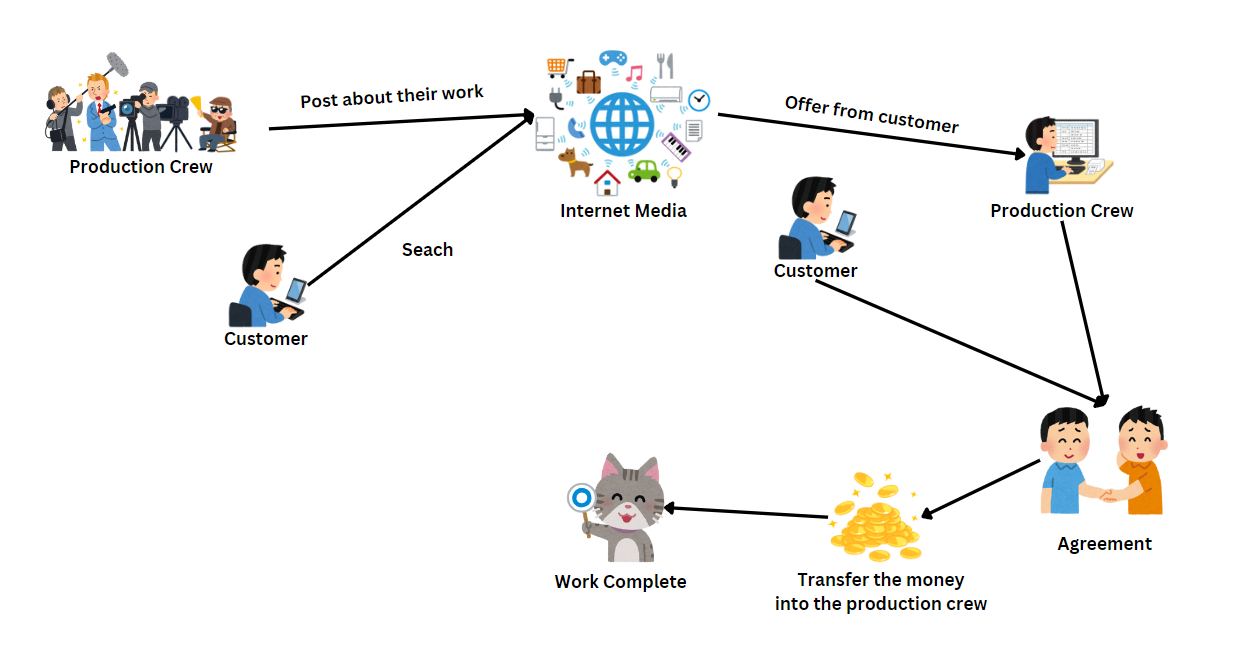
\includegraphics[width=0.9\textwidth]{asis.png}
\end{frame}

\subsection{To-be System Overview}
\begin{frame}{To-be System Overview}
    \centering
    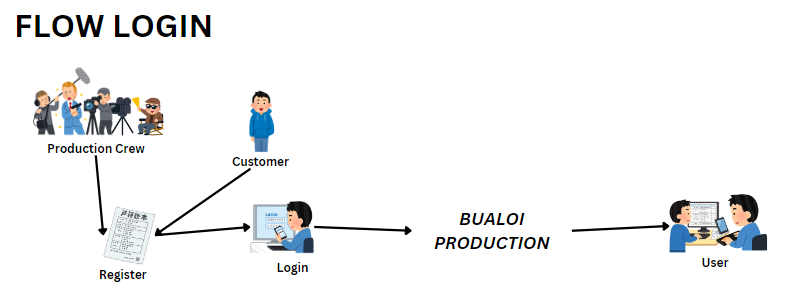
\includegraphics[width=\textwidth]{flowlogin.png}


\end{frame}

\begin{frame}{To-be System Overview}
    \centering
    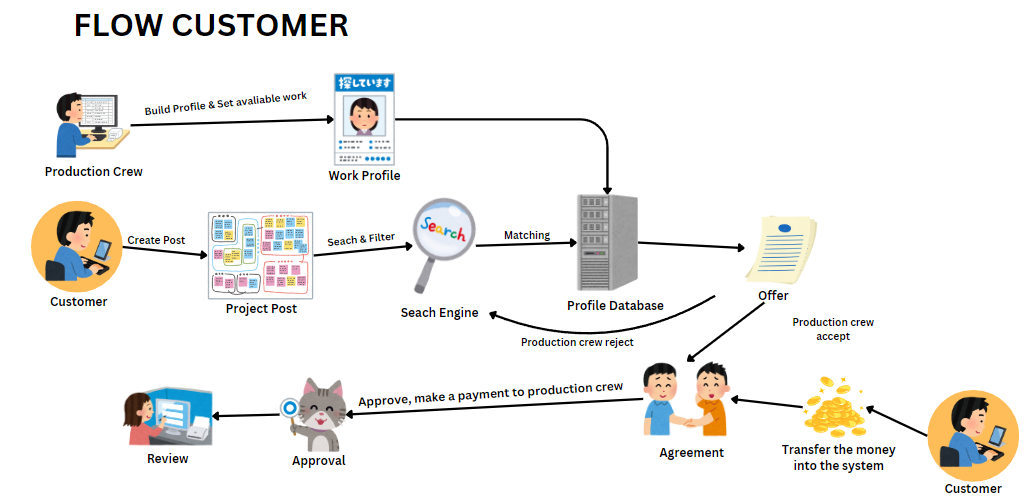
\includegraphics[width=0.85\textwidth]{flowcustomer.png}
\end{frame}
\begin{frame}{To-be System Overview}
    \centering
    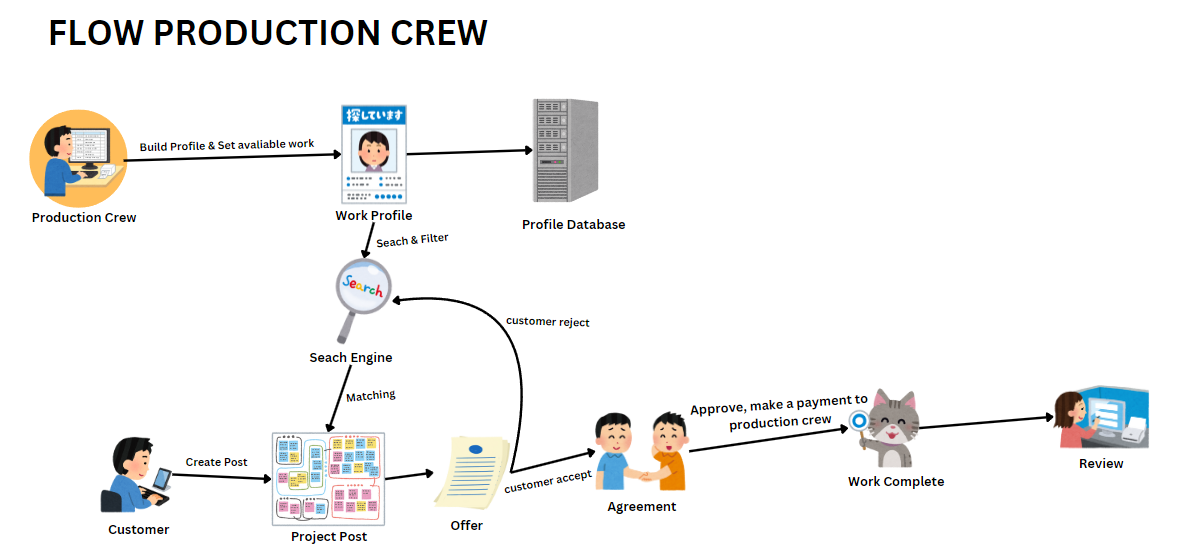
\includegraphics[width=0.75\textwidth]{flowerproductioncrew.png}
\end{frame}


\subsection{Constraints}
\begin{frame}{Constraints}
    \begin{enumerate}
        \item The system can be deployed by March 31, 2025.
        \item The system must be compatible with all web browsers, including smartphones.
        \item The system must comply with the Personal Data Protection Act (PDPA).
        \item The system must ensure secure payment transactions through reliable payment channels.
        \item The system must be able to accommodate a growing user base.
        \item There must be a system for verifying and validating the identity of media production teams and media producers.
    \end{enumerate}
\end{frame}

\section{Scope of the project}
\subsection{Functional Requirements}

\begin{frame}{Functional Requirements}
    \begin{alertblock}{User Management}
        \begin{enumerate}
            \item Identity verification and account management system.
            \item Admin system
            \item Support system
            \item Notification system
        \end{enumerate}
    \end{alertblock}

\end{frame}

\begin{frame}{Functional Requirements}
    \begin{block}{User Interaction}
        \begin{enumerate}
            \item Posting system
            \item Project history system
            \item Search and Filtering system
            \item Review system
        \end{enumerate}
    \end{block}
    \begin{exampleblock}{Product \& Transactions}
        \begin{enumerate}
            \item Payment system
            \item Subscription system.
        \end{enumerate}
    \end{exampleblock}
\end{frame}

\subsection{Non-Functional Requirements}
\begin{frame}{Non-Functional Requirements}
    \centering \resizebox{0.75\textwidth}{!}{
        \begin{columns}
            \begin{column}{0.5\textwidth}
                \begin{block}{Operational Requirements}
                    \begin{enumerate}
                        \item The system must be connected to the internet.
                        \item The system must be responsive web application.
                        \item The system must automatically back up the database every 6 hours.
                        \item The system must be accessible from modern browsers on both desktop and mobile devices.
                        \item The system must support both real-time and asynchronous communication between users.
                    \end{enumerate}
                \end{block}
            \end{column}
            \begin{column}{0.5\textwidth}
                \begin{block}{Performance Requirements}
                    \begin{enumerate}
                        \item The system must respond within 1 second after user interaction.
                        \item The system must support up to 10,000 concurrent users.
                        \item The search and filtering functions must return results within 3 seconds for up to 1,000 profiles.
                        \item The platform must process payments within 5 seconds.
                        \item Project match suggestions must be displayed within 5 seconds after posting a job.
                    \end{enumerate}
                \end{block}
            \end{column}
        \end{columns}
    }
\end{frame}

\begin{frame}{Non-Functional Requirements}
    \centering \resizebox{0.75\textwidth}{!}{
        \begin{columns}
            \begin{column}{0.5\textwidth}
                \begin{block}{Security Requirements}
                    \begin{enumerate}
                        \item The system must provide multi-factor authentication for account verification, especially for media production professionals.
                        \item The system must record and track all changes made to sensitive data (e.g., profiles, payment information).
                        \item User data must be anonymized if the account is deleted and retained for no longer than 6 months.
                    \end{enumerate}
                \end{block}
            \end{column}
            \begin{column}{0.5\textwidth}
                \begin{block}{Cultural and Political Requirements}
                    \begin{enumerate}
                        \item The system must be available in both English and Thai.
                        \item The system must comply with local privacy laws, such as the PDPA (Personal Data Protection Act) for Thailand, and GDPR for users worldwide.
                        \item The system must allow users to specify their preferred language for communication.
                    \end{enumerate}
                \end{block}
            \end{column}
        \end{columns}
    }
\end{frame}

\begin{frame}{Non-Functional Requirements}
    \centering \resizebox{0.8\textwidth}{!}{
        \begin{columns}
            \begin{column}{0.5\textwidth}
                \begin{block}{Reliability Requirements}
                    \begin{enumerate}
                        \item The system must have an uptime of at least 99.9%.
                        \item The system must guarantee zero data loss by continuously backing up critical data every 6 hours.
                        \item The platform must be able to handle peak traffic periods through load balancing.

                    \end{enumerate}
                \end{block}
            \end{column}
            \begin{column}{0.5\textwidth}
                \begin{block}{Usability Requirements}
                    \begin{enumerate}
                        \item The system interface must be user-friendly, requiring no more than 2 clicks to navigate between main features (e.g., posting jobs, sending messages).
                        \item The platform must include onboarding and tutorials for new users, explaining how to post jobs, search for talent, and review past projects.
                        \item The review and feedback system must be easy to use and available immediately after a project is marked as completed.

                    \end{enumerate}
                \end{block}
            \end{column}
        \end{columns}
    }
\end{frame}


\begin{frame}{Non-Functional Requirements}
    \centering \resizebox{0.8\textwidth}{!}{
        \begin{columns}
            \begin{column}{0.5\textwidth}
                \begin{block}{Scalability Requirements}
                    \begin{enumerate}
                        \item The system must be designed to scale horizontally to accommodate future growth in the number of users and transactions.
                        \item The platform must support dynamic scalability during periods of high demand without impacting the user experience.
                    \end{enumerate}
                \end{block}
            \end{column}
            \begin{column}{0.5\textwidth}
                \begin{block}{Privacy Requirements}
                    \begin{enumerate}
                        \item The system must implement user-controlled privacy settings to determine which information (e.g., profiles, work history) is public or private.
                        \item Personal data must be stored and processed in accordance with relevant privacy regulations.
                        \item The system must allow users to download and delete their data upon request.
                    \end{enumerate}
                \end{block}
            \end{column}
        \end{columns}
    }
\end{frame}

\begin{frame}{Non-Functional Requirements}

    \begin{block}{Maintainability Requirements}
        \begin{enumerate}
            \item The system must be modular to facilitate easy updates and the addition of new features.
            \item The platform's codebase must adhere to standard coding practices to ensure maintainability and supportability.
            \item Documentation must be provided for both developers and users, outlining how to use and customize the system.
        \end{enumerate}
    \end{block}
\end{frame}

\section{The selected SDLC methodology and rationale}
\subsection{SDLC Method}
\begin{frame}{SDLC Method}
    Throwaway prototyping \\
    Reasons:
    \begin{enumerate}
        \item Using unfamiliar technology.
        \item The system design is complex.
        \item User requirements are unclear.
        \item The system must be reliable.
    \end{enumerate}


\end{frame}

\subsection{Work Breakdown Structure}
\begin{frame}{Work Breakdown Structure}

    \centering
    \resizebox{0.9\textwidth}{!}{
        \begin{tabular}{|c|l|c|c|c|}
            \hline
            Task Number & Task Name               & Duration (days) & Dependency & Status   \\
            \hline
            1           & Planning                & 7               & -          & Complete \\
            2           & Analysis                & 15              & 1          & Complete \\
            3           & Analysis Iteration 1    & 9               & 2          & Open     \\
            4           & Design Iteration 1      & 11              & 3          & Open     \\
            5           & Implement Iteration 1   & 7               & 4          & Open     \\
            6           & Analysis Iteration 2    & 9               & 5          & Open     \\
            7           & Design Iteration 2      & 13              & 6          & Open     \\
            8           & Implement Iteration 2   & 7               & 7          & Open     \\
            9           & Analysis Iteration 3    & 6               & 8          & Open     \\
            10          & Design Iteration 3      & 10              & 9          & Open     \\
            11          & Implement Iteration 3   & 7               & 10         & Open     \\
            12          & Design Final System     & 7               & 11         & Open     \\
            13          & Implement Final System  & 55              & 12         & Open     \\
            14          & Deliver finished system & -               & 13         & Open     \\
            \hline
        \end{tabular}
    }

\end{frame}
\subsection{Gnatt Chart}

\begin{frame}
    \begin{figure}[!htp]
        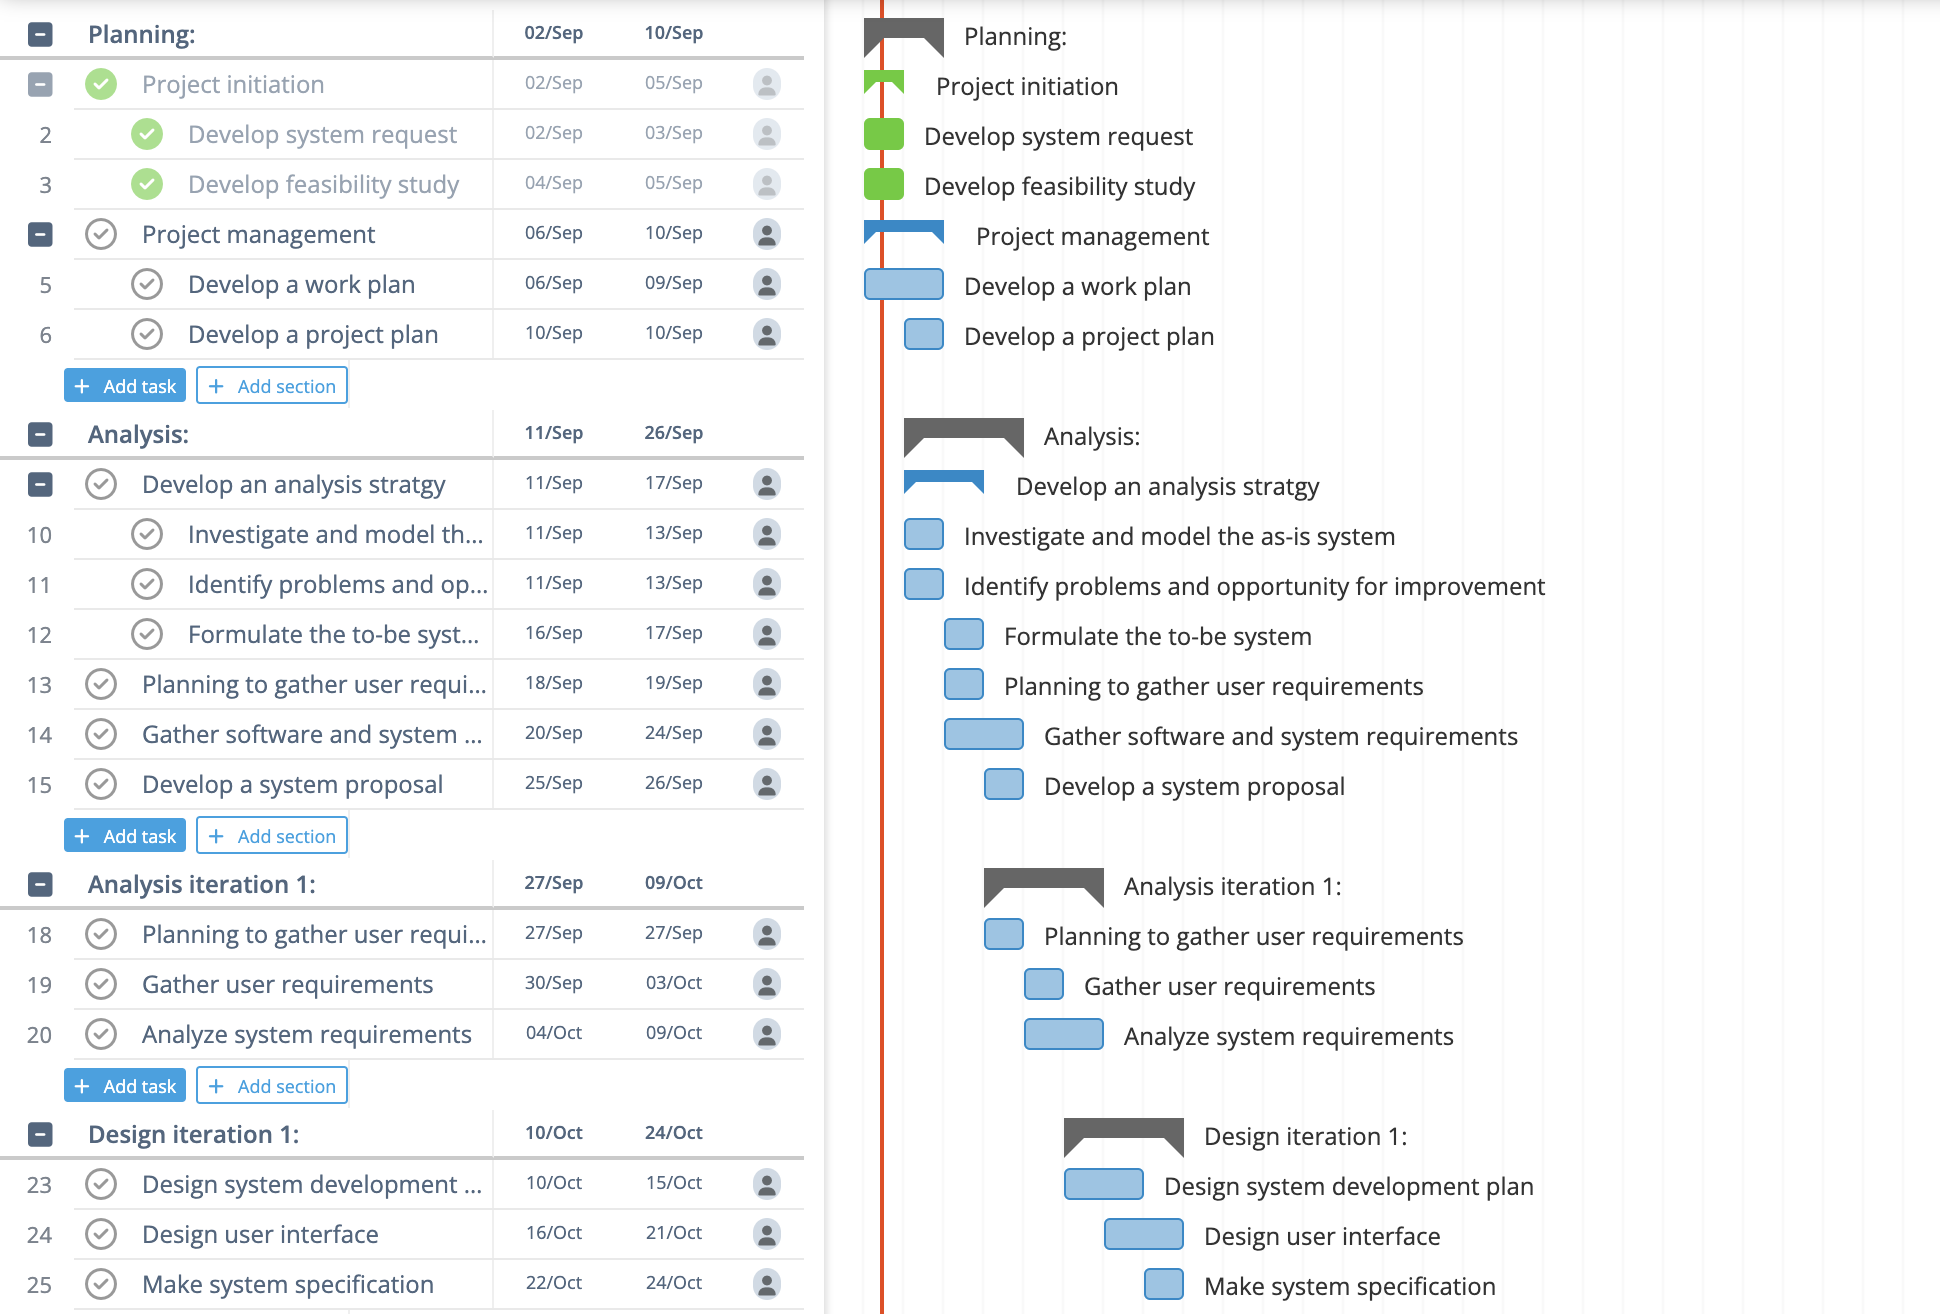
\includegraphics[width=0.6\textwidth]{Gnatt1.png}
        \caption{Planning - Design iteration 1}
    \end{figure}
\end{frame}

\begin{frame}
    \begin{figure}[!htp]
        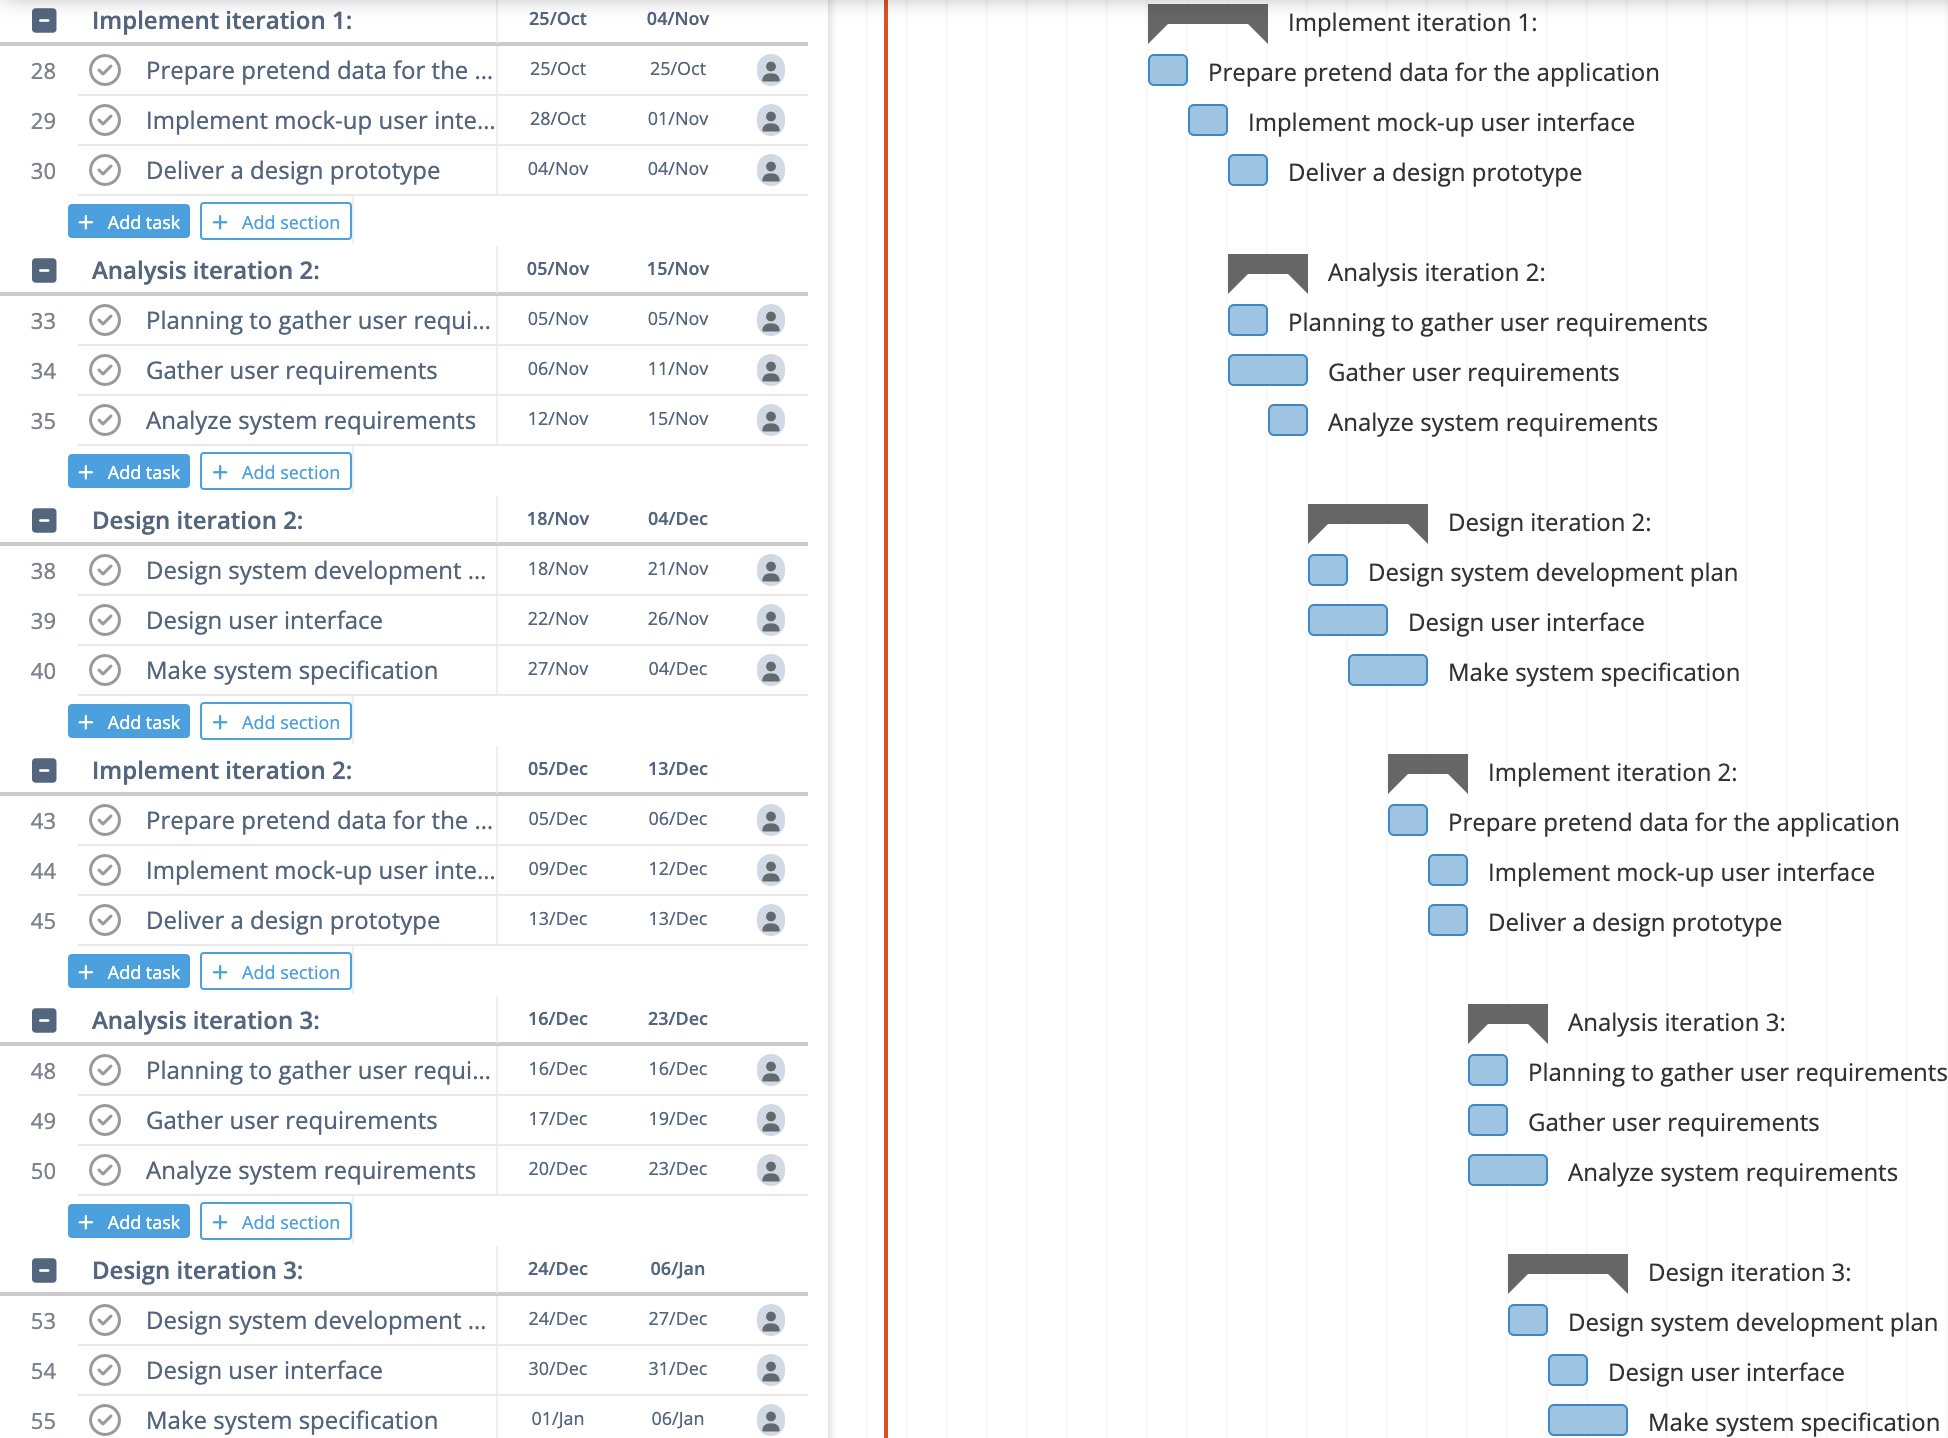
\includegraphics[width=0.6\textwidth]{Gnatt2.png}
        \caption{Implement iteration 1 - Design iteration 3}
    \end{figure}
\end{frame}

\begin{frame}
    \begin{figure}[!htp]
        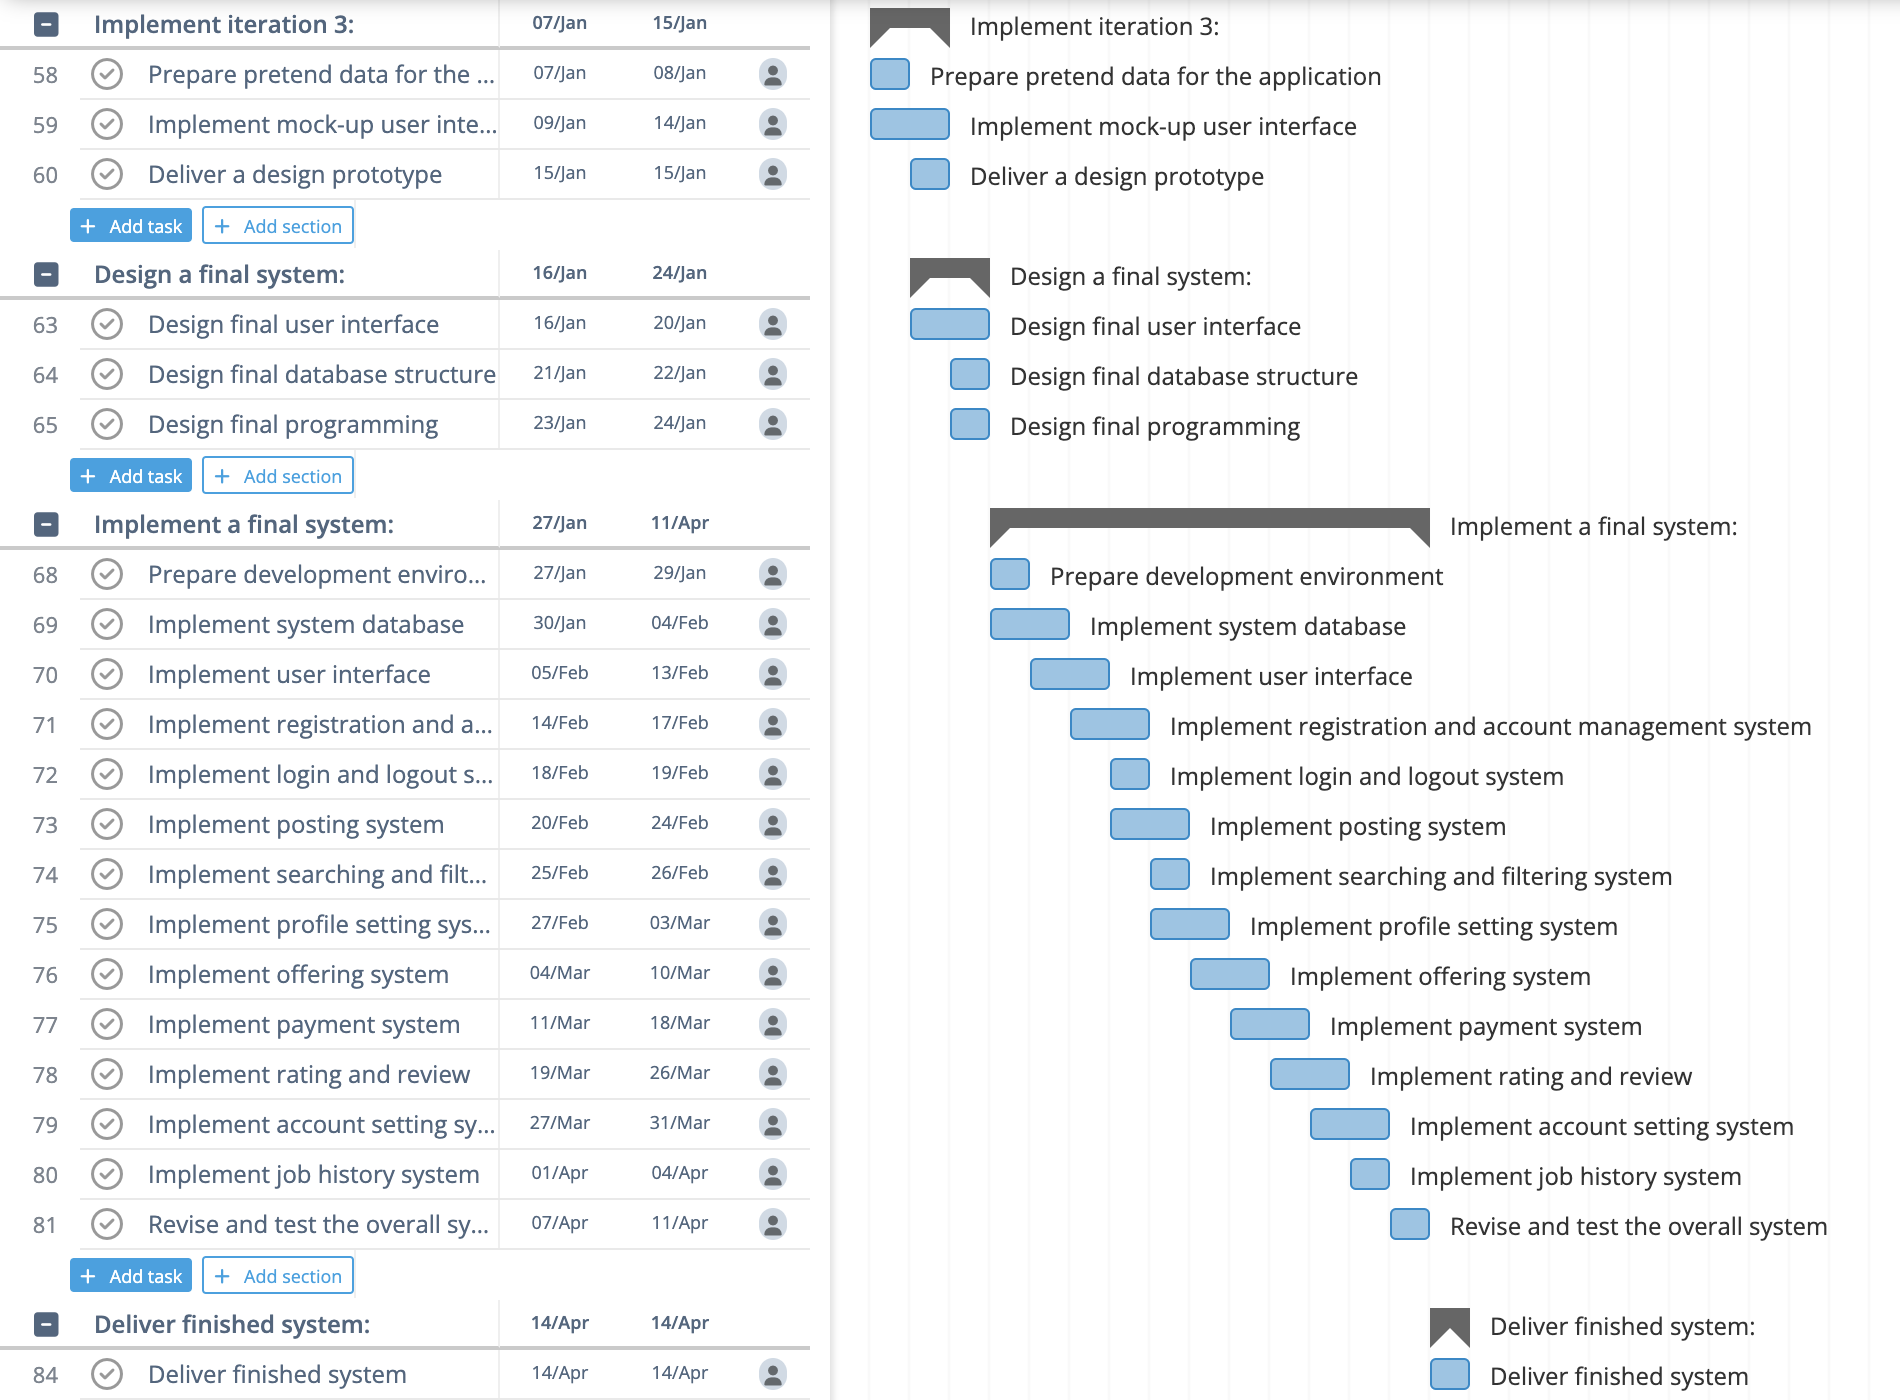
\includegraphics[width=0.6\textwidth]{Gnatt3.png}
        \caption{Implement iteration 3 - Deliver finished system}
    \end{figure}
\end{frame}

\subsection{Cost Estimation}

\begin{frame}{Cost Estimation}
    \centering
    \resizebox{0.9\textwidth}{!}{
        \begin{tabular}{|l|p{7cm}|c|c|c|}
            \hline
            Task                   & Responsible Role                                                                            & Effort (person-months) & Average Labor Rate (Baht/Month) & Labor Cost       \\
            \hline
            Planning               & Project Manager, System Analyst                                                             & 0.38                   & 87,500                          & 33,415           \\
            \hline
            Analysis               & Project Manager, System Analyst, Business Analyst, Infrastructure Analyst, Technical Leader & 0.82                   & 94,000                          & 76,923           \\
            \hline
            Analysis Iteration 1   & System Analyst, Infrastructure Analyst                                                      & 0.49                   & 94,000                          & 46,154           \\
            \hline
            Design Iteration 1     & System Analyst, Infrastructure Analyst                                                      & 0.6                    & 62,500                          & 37,507           \\
            \hline
            Implement Iteration 1  & Software Developer                                                                          & 0.38                   & 40,000                          & 15,276           \\
            \hline
            Analysis Iteration 2   & Project Manager, System Analyst, Business Analyst, Infrastructure Analyst, Technical Leader & 0.49                   & 94,000                          & 46,154           \\
            \hline
            Design Iteration 2     & System Analyst, Infrastructure Analyst                                                      & 0.71                   & 62,500                          & 44,326           \\
            \hline
            Implement Iteration 2  & Software Developer                                                                          & 0.38                   & 40,000                          & 15,276           \\
            \hline
            Analysis Iteration 3   & Project Manager, System Analyst, Business Analyst, Infrastructure Analyst, Technical Leader & 0.33                   & 94,000                          & 30,769           \\
            \hline
            Design Iteration 3     & System Analyst, Infrastructure Analyst                                                      & 0.55                   & 62,500                          & 34,097           \\
            \hline
            Implement Iteration 3  & Software Developer                                                                          & 0.38                   & 40,000                          & 15,276           \\
            \hline
            Design Final System    & System Analyst, Infrastructure Analyst, Quality Assurance                                   & 0.38                   & 75,000                          & 28,642           \\
            \hline
            Implement Final System & Software Developer, Quality Assurance                                                       & 3                      & 63,333                          & 190,034          \\
            \hline
            \textbf{Total}         &                                                                                             & \textbf{8.89}          &                                 & \textbf{613,847} \\
            \hline
        \end{tabular}
    }
\end{frame}

\begin{frame}{Cumulative NPV Over Time}
    \centering
    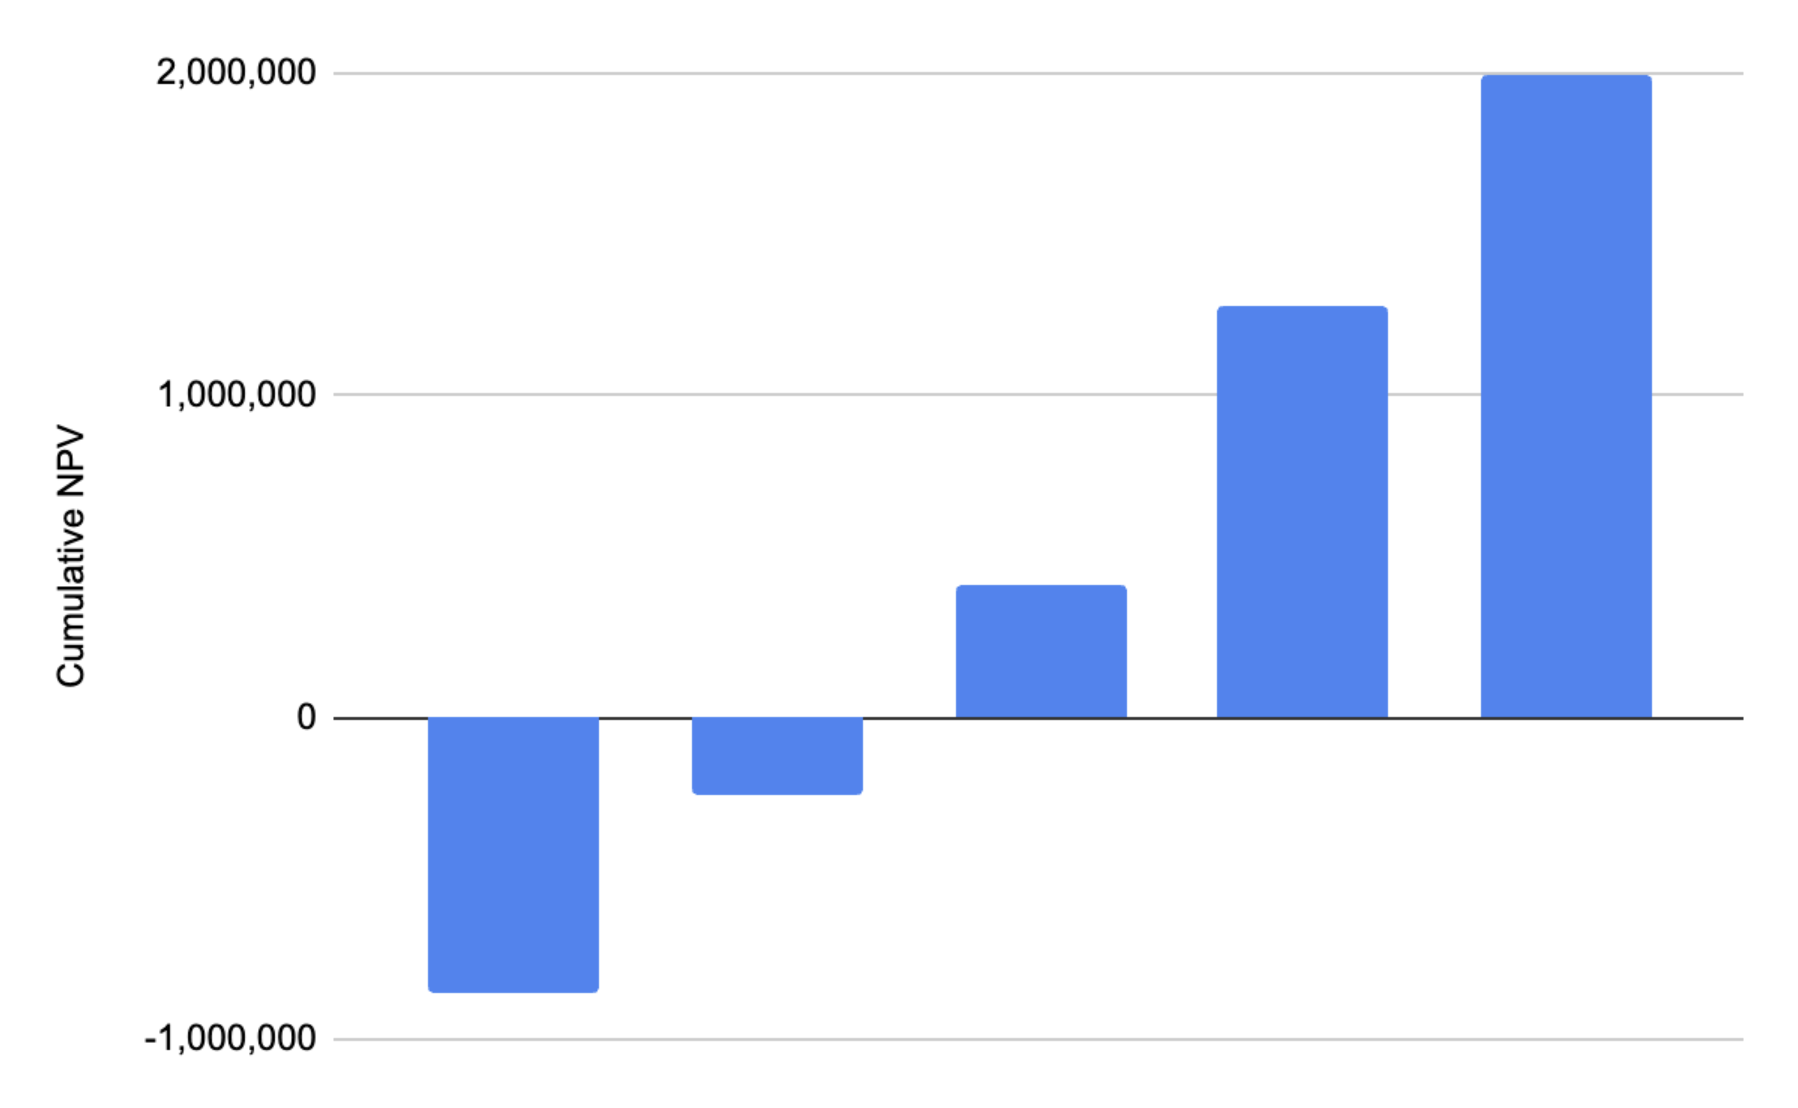
\includegraphics[width=0.6\textwidth]{barchart.png}
    \\
    ROI: 108.42\% \\
    Break Even Point: 2.3 Years

\end{frame}

\begin{frame}{Development Cost}
    \centering
    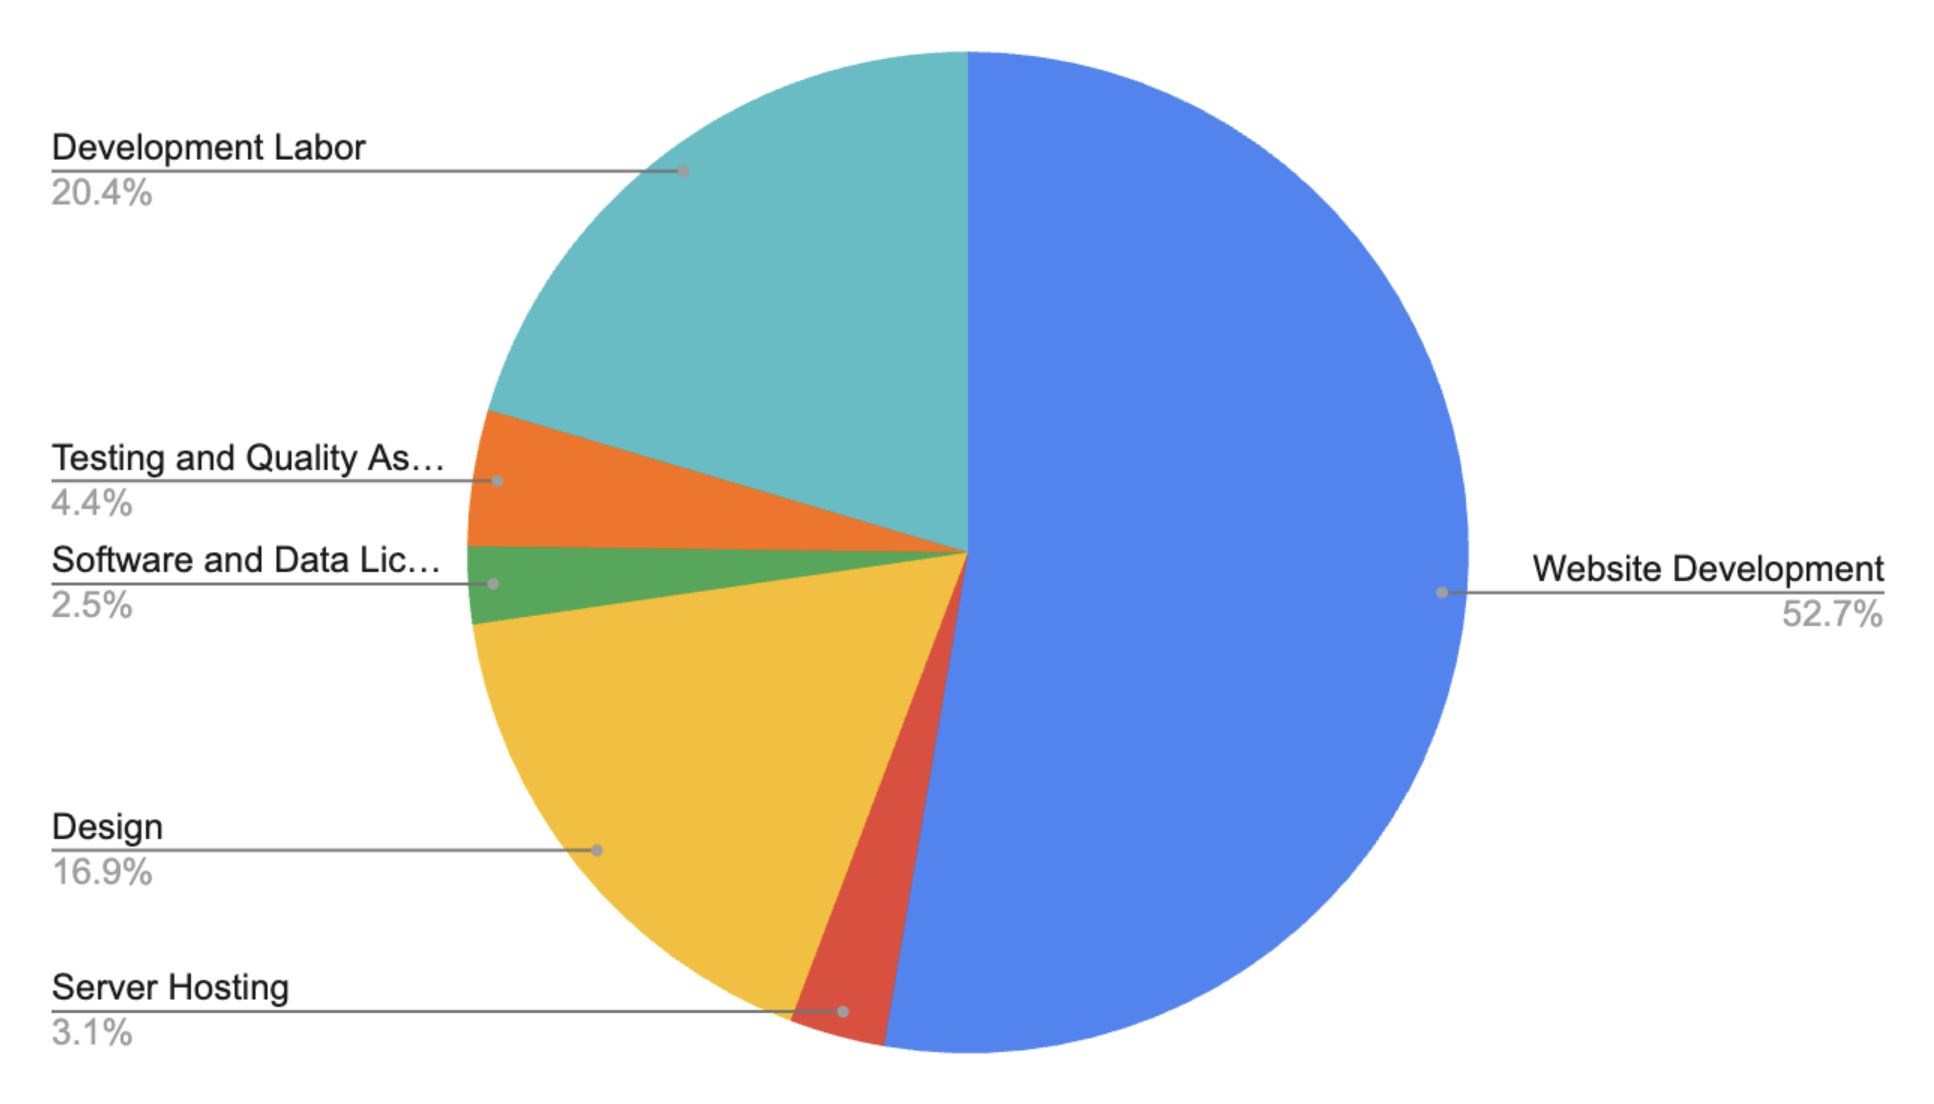
\includegraphics[width=0.6\textwidth]{developmentcost.png}

\end{frame}

\begin{frame}{Operational Cost}
    \centering
    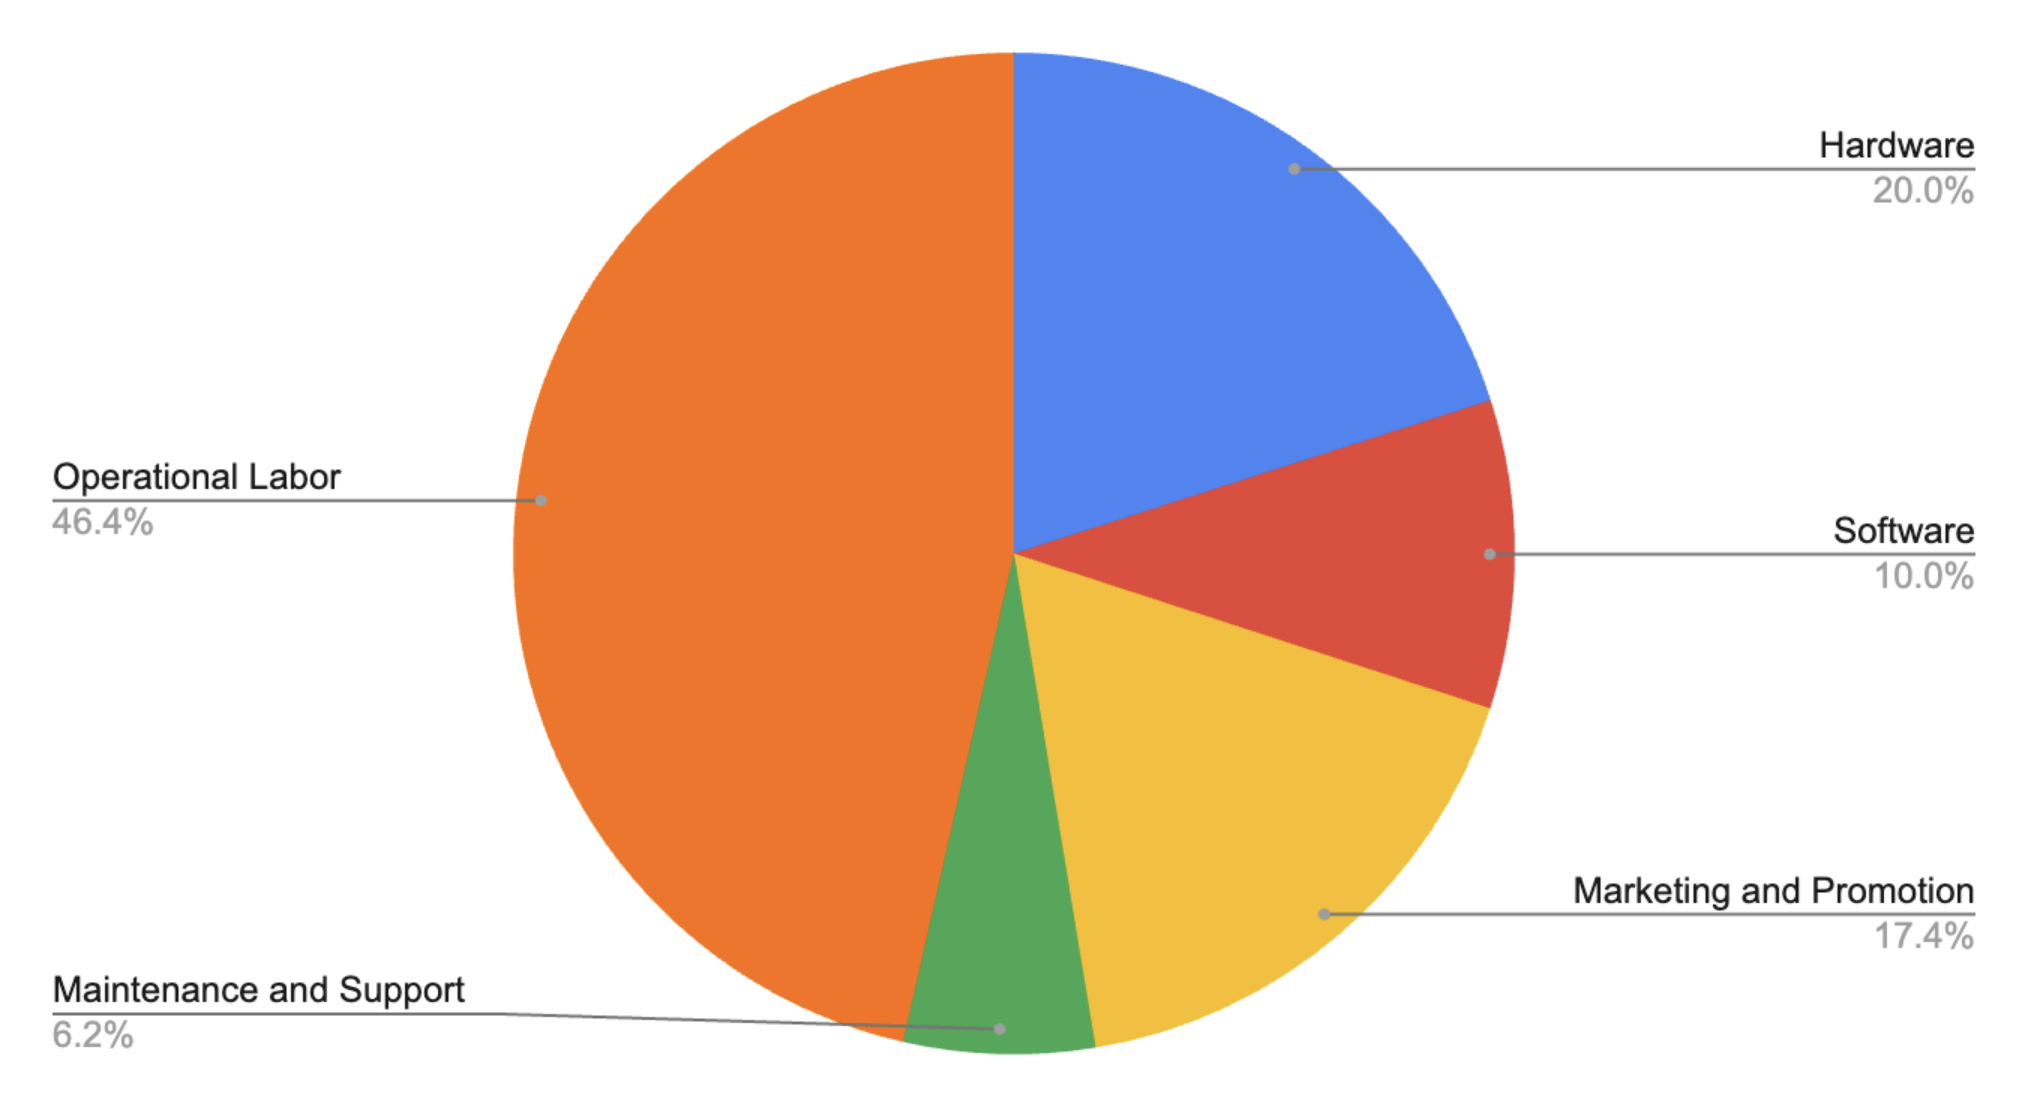
\includegraphics[width=0.6\textwidth]{OperationalCost.png}

\end{frame}

\begin{frame}{Income}
    \centering
    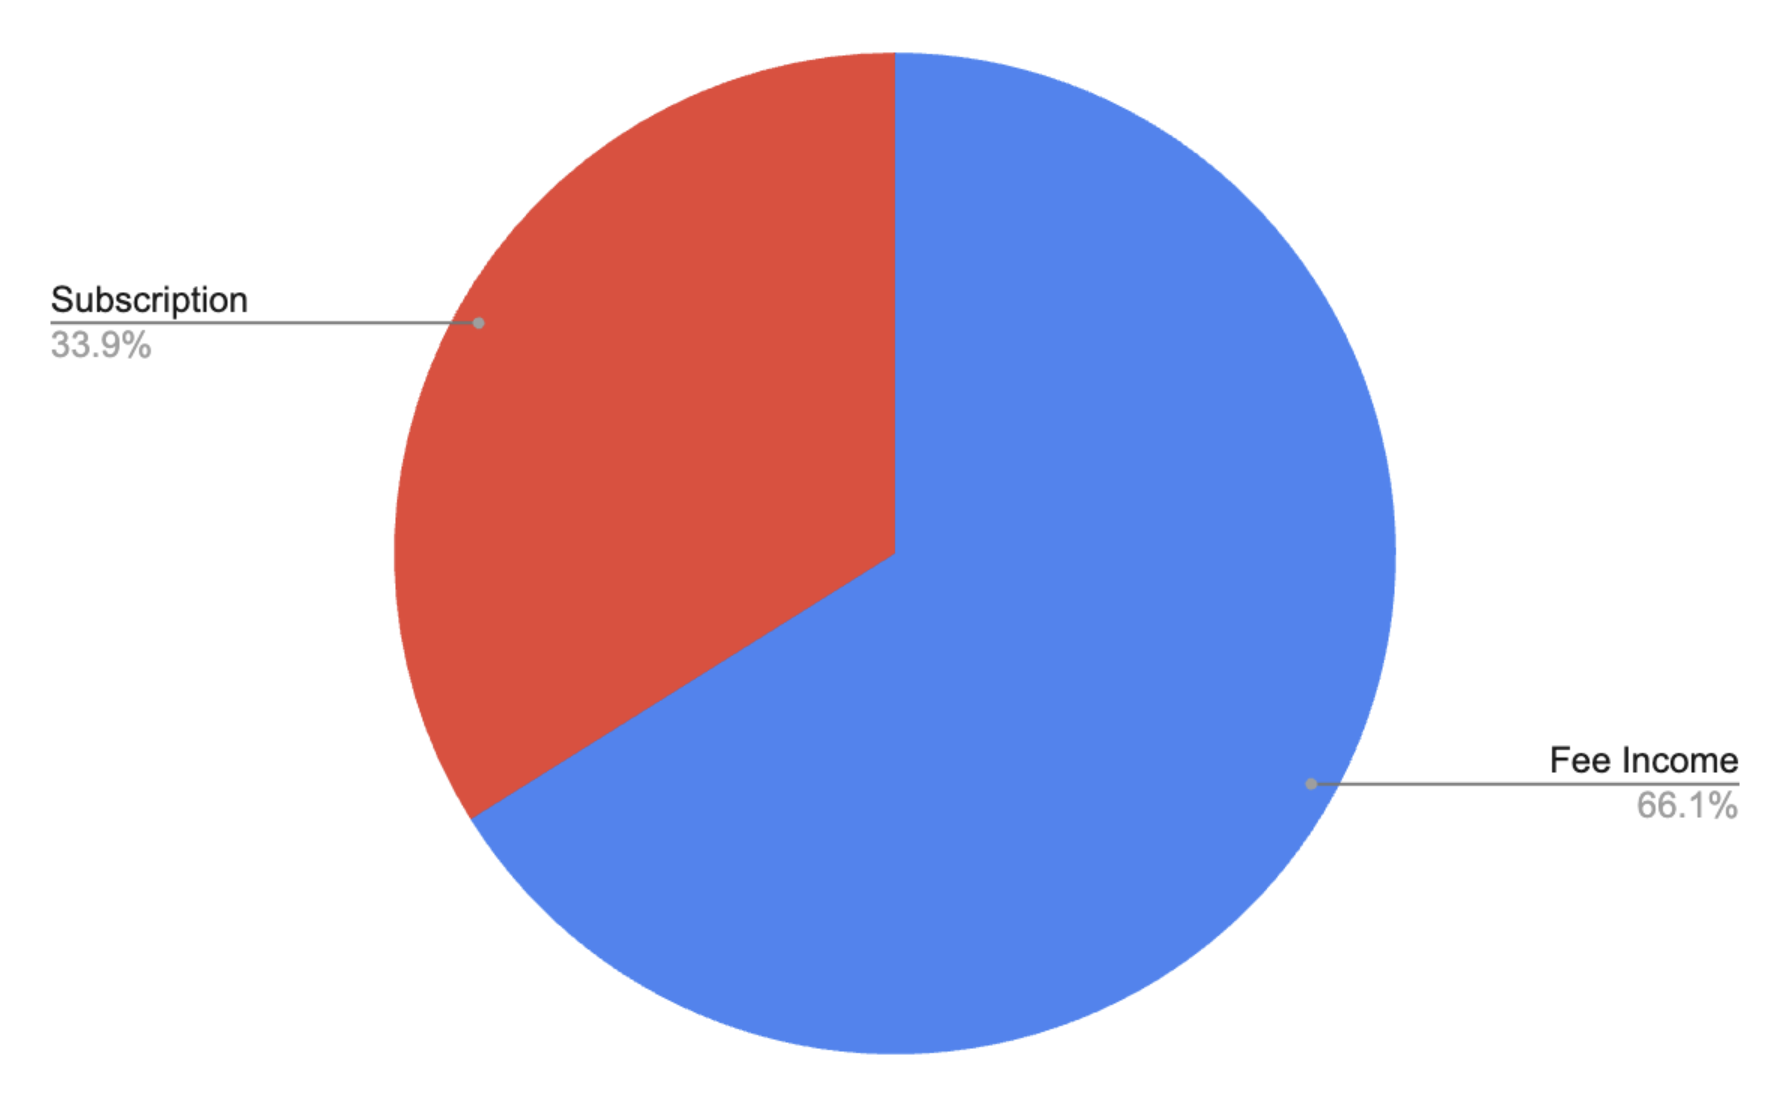
\includegraphics[width=0.6\textwidth]{Income.png}

\end{frame}

\section{The Benefits of the Project}
\subsection{Benefits}

\begin{frame}{Benefits}{Production crew}
    \begin{enumerate}
        \item Gained opportunities to reach new customers.
        \item Media production professionals become more recognized.
        \item Build credibility and trust with media producers.
    \end{enumerate}
\end{frame}

\begin{frame}{Benefits}{Customer}
    \begin{enumerate}
        \item Access a team of media production professionals with experience and skills in a variety of fields.
        \item Save time in finding suitable media production professionals.
        \item Access reviews and feedback from other media producers, which helps in assessing the quality and reliability of media production professionals.
    \end{enumerate}
\end{frame}

\begin{frame}{Benefits}{Bualoi Production}
    \begin{enumerate}
        \item Enhancing the database with profiles of media professionals and producers will help attract new users to the platform.
        \item Collecting data on user behavior will enable administrators to analyze marketing strategies and plan future projects effectively.
        \item Generate revenue through subscription fees and commissions from transactions.
    \end{enumerate}
\end{frame}

\section{Appendix}
\subsection{Technical Feasibility}
\begin{frame}{Technical Feasibility}
    \centering
    \resizebox{\textwidth}{!}{
        \begin{tabular}{|c|p{10cm}|c|}
            \hline
            Section         & Detail                                                                                                                                                                                                   & Risk        \\
            \hline
            Functional Area & The team understands and is familiar with how media production teams currently operate, but may still need additional information about specific processes to further develop the platform's efficiency. & Low         \\
            \hline
            Technology      & The development team has general web development skills, but building complex systems like banking transactions will take more time.                                                                     & Medium      \\
            \hline
            Project Size    & There are 10 key requirements, and the development team consists of 9 members, with a development timeline of 4 months.                                                                                  & Low-Medium  \\
            \hline
            Compatibility   & Financial transactions and identity verification add complexity and raise security concerns.                                                                                                             & Medium-High \\
            \hline
        \end{tabular}
    }
    $\newline$
    Overall Risk: \textbf{Medium}
\end{frame}

\subsection{Economic Feasibility}
\begin{frame}{Economic Feasibility}
    \centering
    \resizebox{0.65\textwidth}{!}{
        \begin{tabular}{|l|l|l|c|c|c|c|}
            \hline
                                           & 2024                                & 2025      & 2026      & 2027      & 2028      & Total              \\
            \hline
            \textbf{Income}                &                                     &           &           &           &           &                    \\
            \hline
            Fee Income                     & 0                                   & 696,000   & 800,100   & 791,500   & 837,200   &                    \\
            \hline
            Subscription                   & 0                                   & 350,100   & 426,900   & 447,100   & 409,000   &                    \\
            \hline
            Total Benefits                 & 0                                   & 1,046,100 & 1,227,000 & 1,238,600 & 1,246,200 & \textbf{4,071,818} \\
            \hline
            PV of Benefits                 & 0                                   & 957,945   & 1,075,216 & 1,038,642 & 1,000,014 &                    \\
            \hline
            PV of All Benefits             & 0                                   & 957,945   & 2,033,161 & 3,071,803 & 4,071,818 &                    \\
            \hline
            \textbf{Development Costs}     &                                     &           &           &           &           &                    \\
            \hline
            Website Development            & 358,939                             & 0         & 0         & 0         & 0         &                    \\
            \hline
            Server Hosting                 & 21,000                              & 0         & 0         & 0         & 0         &                    \\
            \hline
            Design                         & 115,390                             & 13,000    & 0         & 0         & 0         &                    \\
            \hline
            Software and Data Licenses     & 17,000                              & 0         & 0         & 0         & 0         &                    \\
            \hline
            Testing and Quality Assurance  & 30,000                              & 15,000    & 15,900    & 16,854    & 17,865    &                    \\
            \hline
            Development Labor              & 138,980                             & 105,000   & 120,000   & 0         & 0         &                    \\
            \hline
            Total Development Costs        & 681,309                             & 133,000   & 135,900   & 16,854    & 17,865    &                    \\
            \hline
            \textbf{Operational Costs}     &                                     &           &           &           &           &                    \\
            \hline
            Hardware                       & 42,300                              & 65,600    & 65,600    & 65,600    & 65,600    &                    \\
            \hline
            Software                       & 21,000                              & 21,000    & 21,000    & 21,000    & 21,000    &                    \\
            \hline
            Marketing and Promotion        & 36,700                              & 24,800    & 26,300    & 27,800    & 29,500    &                    \\
            \hline
            Maintenance and Support        & 13,000                              & 13,780    & 14,606    & 15,483    & 16,412    &                    \\
            \hline
            Operational Labor              & 98,000                              & 103,880   & 110,112   & 116,719   & 123,722   &                    \\
            \hline
            Total Operational Costs        & 211,000                             & 229,060   & 237,618   & 246,602   & 256,234   &                    \\
            \hline
            Total Costs                    & 892,309                             & 362,060   & 373,518   & 263,456   & 274,099   &                    \\
            \hline
            PV of Costs                    & 853,884                             & 331,549   & 327,313   & 220,924   & 219,951   & \textbf{1,953,621} \\
            \hline
            PV of All Costs                & 853,884                             & 1,185,433 & 1,512,746 & 1,733,670 & 1,953,621 &                    \\
            \hline
            Total Project Benefits - Costs & -892,309                            & 684,040   & 853,482   & 975,144   & 972,101   &                    \\
            \hline
            Yearly NPV                     & -853,884                            & 626,396   & 747,903   & 817,718   & 780,063   & \textbf{2,118,197} \\
            \hline
            Cumulative NPV                 & -853,884                            & -227,488  & 520,415   & 1,338,133 & 2,118,197 &                    \\
            \hline
            \textbf{Return on Investment}  & \textbf{108.42\% (2118197/1953621)} &           &           &           &           &                    \\
            \hline
        \end{tabular}
    }
    \\
    \centering
    $\newline$
    Overall Risk: \textbf{Medium}
\end{frame}

\subsection{Organization Feasibility}
\begin{frame}{Organization Feasibility}
    \centering
    \resizebox{\textwidth}{!}{
        \begin{tabular}{|c|p{10cm}|c|}
            \hline
            Section              & Detail                                                                                                                                                                                                                        & Risk   \\
            \hline
            Strategy Alignment   & The system's goal aligns with the organization's objective of becoming a central platform for matching media production teams and clients.                                                                                    & Low    \\
            \hline
            Stakeholder Analysis & Media producers: Teams such as directors, set designers, and screenwriters lack an online space for finding work, which this system aims to solve. Service users: They will have more options to find media production teams. & Medium \\
            \hline
        \end{tabular}
    }
    $\newline$
    Overall Risk: \textbf{Medium}
\end{frame}

\subsection{Impact on Society}
\begin{frame}{Impact on Society}
    \centering
    \resizebox{\textwidth}{!}{
        \begin{tabular}{|c|p{10cm}|c|}
            \hline
            Section                    & Detail                                                                                                              & Impact   \\
            \hline
            Economic and Global Impact & The platform helps media professionals find more work and promotes creativity from diverse individuals.             & Positive \\
            \hline
            Society Impact             & The platform may increase precarious gig work, which could impact worker's financial stability and quality of life. & Negative \\
            \hline
            Environmental Impact       & Reduce paper usage and deforestation due to the system's digital system.                                            & Positive \\
            \hline
        \end{tabular}
    }
    $\newline$
    Overall Risk: \textbf{Medium}
\end{frame}

\subsection{Team organization}
\begin{frame}{Team organization}
    \begin{enumerate}
        \item \textbf{Nasmeen Islam} - Software Developer
        \item \textbf{Tanadol Jaichuen} - UI/UX Designer, Software Developer
        \item \textbf{Wiroonpuri Silasap} - Technical Leader, Software Developer
        \item \textbf{Kawin Rattanapun} - Business analyst
        \item \textbf{Tanaphom Hirunyathorn} - UI/UX Designer, Software Developer
        \item \textbf{Chawanakorn Auckayachinda} - System Analyst, Software Developer
        \item \textbf{Paponthanai Ounsopa} - Software Developer
        \item \textbf{Nontanun Ausungnoen} - Project Manager
        \item \textbf{Pana Wanitchollakit} - Quality Assurance
    \end{enumerate}
\end{frame}

\end{document}